\documentclass{ContactProject}


%%\newcommand{\draftpaper}{}


\newif\ifaddendum
\ifx\addendumpaper\undefined
  \addendumfalse
\else
  \addendumtrue
\fi

\newif\ifdraft
\ifx\draftpaper\undefined
  \draftfalse
\else
  \drafttrue
\fi



\usepackage{graphicx}
\usepackage{fullpage}
\usepackage{multirow}
\usepackage{tabularx}

\usepackage{isodateo}
\usepackage[british]{babel}

%%\usepackage{draftcopy}

\ifdraft
\usepackage{eso-pic}
\usepackage{graphicx}
\usepackage{color}
\usepackage{type1cm}
\makeatletter
  \AddToShipoutPicture{%
    \setlength{\@tempdimb}{.5\paperwidth}%
    \setlength{\@tempdimc}{.5\paperheight}%
    \setlength{\unitlength}{1pt}%
    \put(\strip@pt\@tempdimb,\strip@pt\@tempdimc){%
      \makebox(0,0){\rotatebox{45}{\textcolor[gray]{0.9}{\fontsize{5cm}{5cm}\selectfont{\bf draft}}}}
    }
}
\makeatother
\fi

%%\usepackage{natbib}
\usepackage{code}
\CodeNoNumber

\newenvironment{codecase}[1]{\subsection{#1}}{}


\usepackage[sort]{natbib}
\newcommand{\citeasnoun}{\citet}
\renewcommand{\cite}{\citep}

\newcommand{\tasect}[1]{ (see Technical Annex, Section~#1)}
%\newcommand{\tasect}[1]{\hfill {\it (Technical Annex, Section #1)}\ \\}

%\emergencystretch=\hsize
\lefthyphenmin=2
\righthyphenmin=2
%\tolerance=9999

%\setcounter {topnumber}{7}
\renewcommand {\topfraction}{0.99}            % common default: 0.8
\renewcommand {\bottomfraction}{0.99}         % common default: 0.8
\setcounter   {totalnumber}{14}               % common default: 3
\renewcommand{\topfraction}{0.999}
\renewcommand {\textfraction}{0.01}           % common default: 0.2
\renewcommand {\floatpagefraction}{0.99}       % common default: 0.5

\newcommand{\dgrs}{$^{\circ}$}
\newcommand{\twiddle}{\char126}
\newcommand{\pflist}
  {     \renewcommand{\labelitemi}{$\triangleright$}
        \setlength{\itemsep}{0mm}
        \setlength{\parsep}{0mm}
        \setlength{\partopsep}{0mm}
        \setlength{\topsep}{0mm}
        \setlength{\parskip}{0mm}    }



\newcommand{\chapquotea}{notset}
\newenvironment{chapquote}[1]{\renewcommand{\chapquotea}{#1}\begin{quote}\it}{{\rm \hspace*{\fill}~\cite[]{\chapquotea} } \end{quote} \noindent}

\newcommand{\righter}[1]{ \hspace*{\fill}~#1}

\newcommand{\activityimage}{notset}

\newenvironment{activity}[2]{ %
  \renewcommand{\activityimage}{#2} %
  \subsubsection*{#1} %
  \begin{tabular}{p{12.5cm}p{3.5cm}} %
    \begin{minipage}{13.5cm} %
      \begin{tabular}{p{1.5cm}p{11.5cm}} %
        \hline %
}{ %
    \\ \hline %
    \end{tabular} %
  \end{minipage} %
  & %
  \begin{minipage}{3.5cm} %
    \raggedleft %
    \includegraphics[height=2cm]{\activityimage} %
  \end{minipage} %
\end{tabular} %
\vspace*{0.1cm} % 
\noindent \\%
}


%\newcommand{\usage}[1]{
%  \noindent
%  \begin{tabular}{|l|}\hline
%  Command: {\bf #1}\\
%\hline\end{tabular}\\
%\noindent}

\newenvironment{packed_itemize}{
\begin{itemize}
  \renewcommand{\labelitemi}{$\triangleright$}
  \setlength{\itemsep}{1pt}
  \setlength{\parskip}{0pt}
  \setlength{\parsep}{0pt}
}{\end{itemize}}

\newcommand{\newusage}{\ \\\noindent\makebox[\textwidth]{\hrulefill}}

\newcommand{\usage}[1]{ \begin{packed_itemize} \item {\it Command:} {\tt #1} \end{packed_itemize}}


\newcommand{\ctt}[1]{{\tt #1}}
\newcommand{\packet}[1]{\framebox{#1}}


\title{Interim Report}

%
%  For one-to-one authur/affil correspondence
\author{Paul Fitzpatrick}


\begin{document}



\deliverable{D1.7}
\title{Exploratory Play Behavior, learning by doing}
\leadpartner{UGDIST}
\revision{1}
\deliverabledate{31/8/2007}
%\submissiondate{15/10/2006}
\disseminationlevel{PU}
\responsible{P. Fitzpatrick}




\maketitle

%%\input{section-front}


\pagenumbering{arabic}

\clearpage
%%%%\tableofcontents
%%%%\clearpage




\section{Introduction}

Exploratory Play Behavior, learning by doing. Artifact tries a fixed
set of actions on a fixed set of objects, learning about the objects
and actions using algorithms of D1.5 and D1.6.



\clearpage

\section{Manipulation: exploring the environments to learn}

\label{sect:manipulation}

IST has continued working on the acquisition and usage of affordance
knowledge (see Deliverable 1.6). The work has focused on two different
directions: (i) the extension of the Bayesian network model described
in Deliverable 1.6 for unsupervised learning of  affordances through
self-exploration; and (ii) the use of this knowledge in imitation
context to learn through observation.

\subsection{Affordance acquisition}
As described in previous documents, we have proposed a general
framework for affordance acquisition based on Bayesian networks. The
robot is able to build through exploration a network describing the
relations between its actions, the object features and the resulting
effects of the action. In the last months, we have completed the set
of experiments to validate the Bayes network affordance model. More
precisely, we have shown how extra features help to disambiguate
situations and improve the prediction capabilities of the
model. Figure~\ref{fig:manipulation:affordances}(a) shows the playground used in the experiments and
Figure~\ref{fig:manipulation:affordances}(b) shows the resulting network.

For instance, the difference of touch and tap on a ball is clear when
applied to objects that roll such as a ball. However, when tapping or
touching a box-like object, the resulting effects are the same. In
this case, it is important to add proprioceptive features such as
contact information to dissambiguate both cases. By using this
proprioceptive information, the robot is able to improve the model of
the world. Figure~\ref{fig:manipulation:affordances}(c) compares the action recognition ratio using a
model with contact information (Figure~\ref{fig:manipulation:affordances}(b)) and a model without this
information.
This work has been published in \cite{montesano:etal:2007}.

\begin{figure}
\begin{tabular}{ccc}
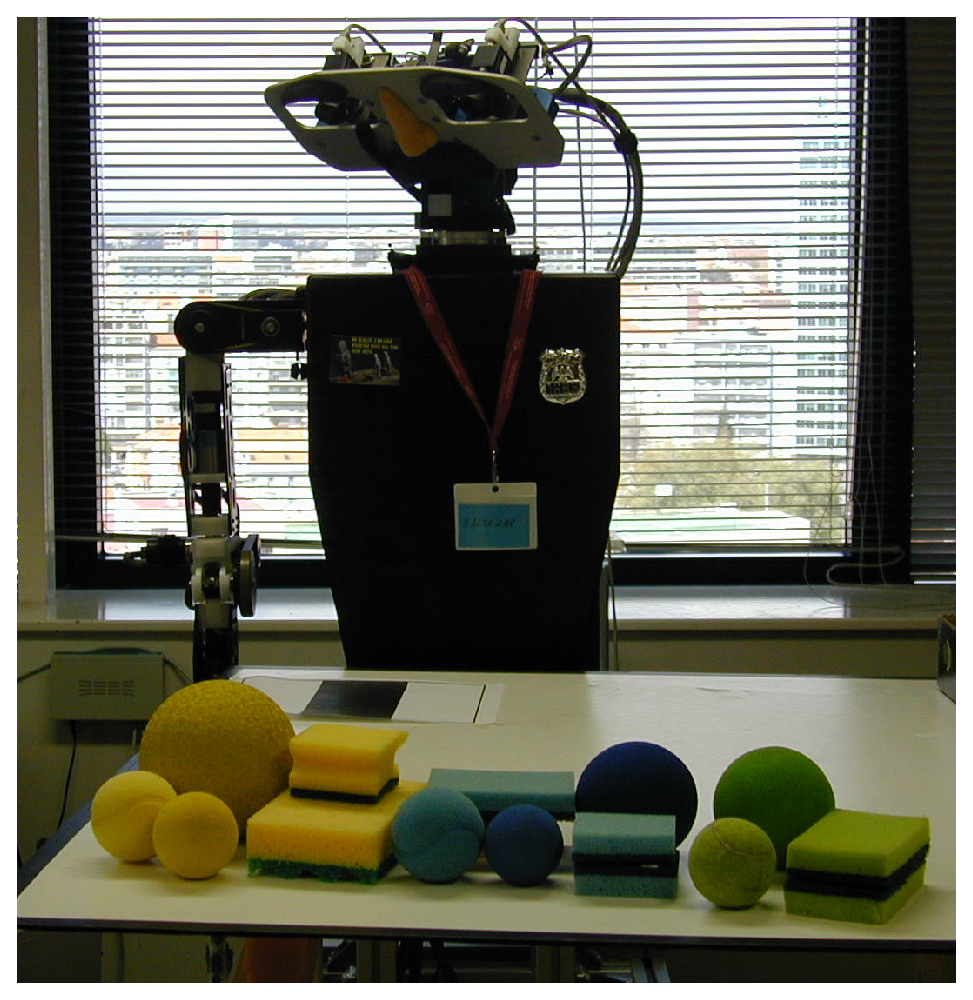
\includegraphics[width=0.3\columnwidth]{images/setup.eps} &
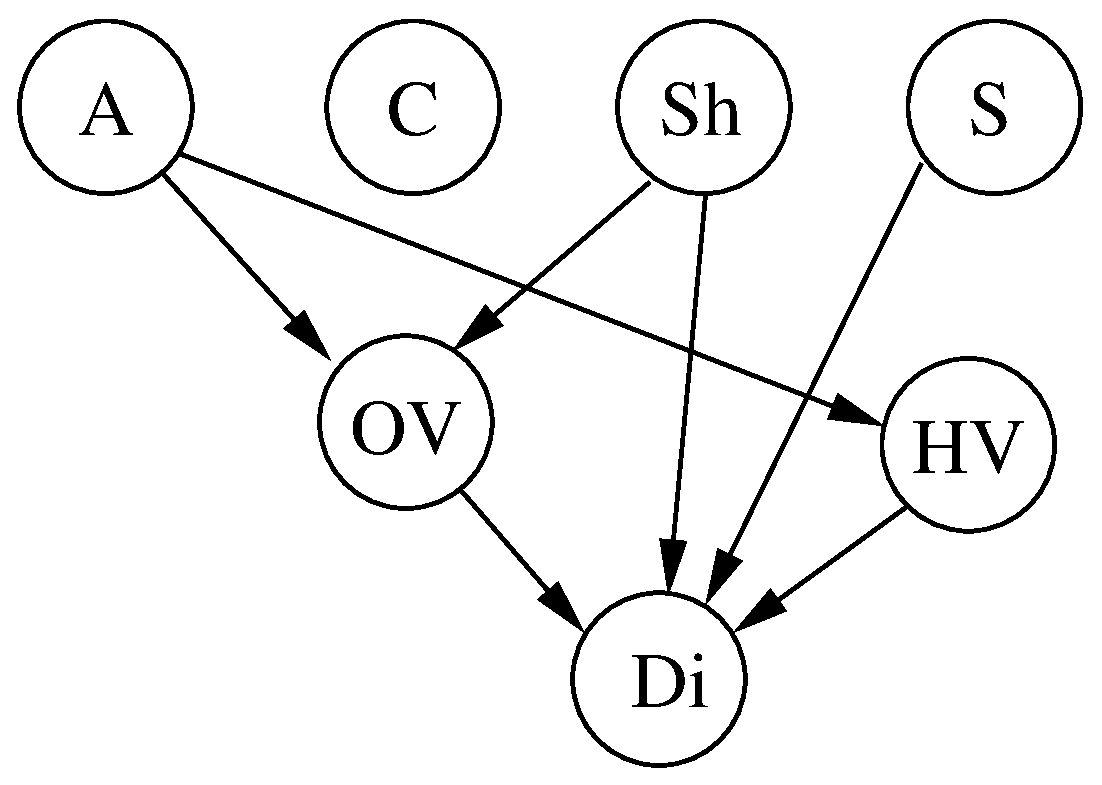
\includegraphics[width=0.3\columnwidth]{images/MCMCIROS1_p072.eps} &
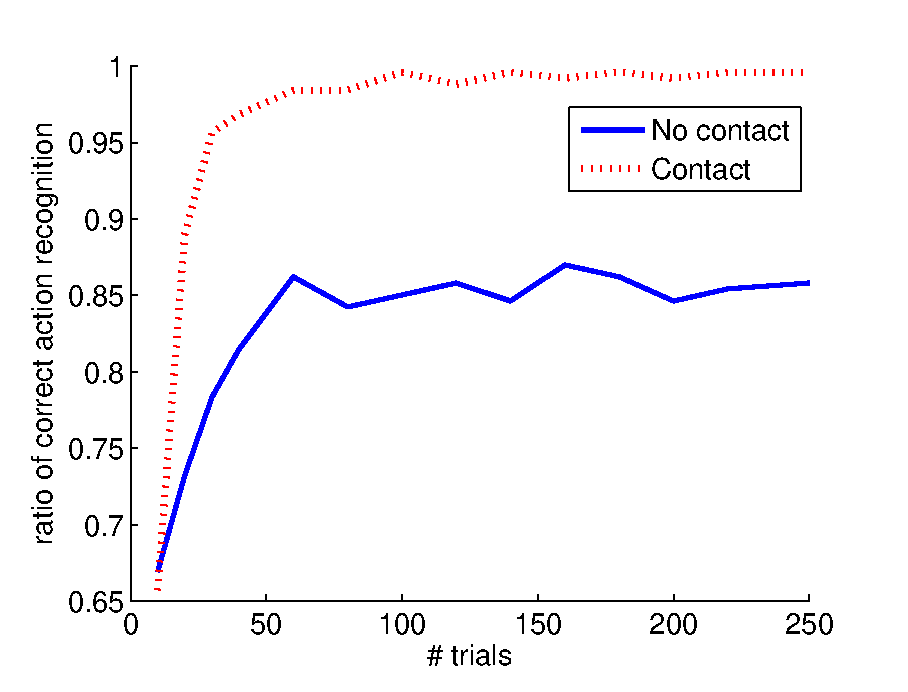
\includegraphics[width=0.3\columnwidth]{images/resIROSActionRecog.eps} \\
(a) & (b) & (c) \\
\end{tabular}
% Figure 5
\caption{(a) Playground for affordance acquisition, (b) Affordance
  network learnt,  (c) ratio of action recognition w/o contact
  information.}
\label{fig:manipulation:affordances}
\end{figure}


\begin{figure}
\centering
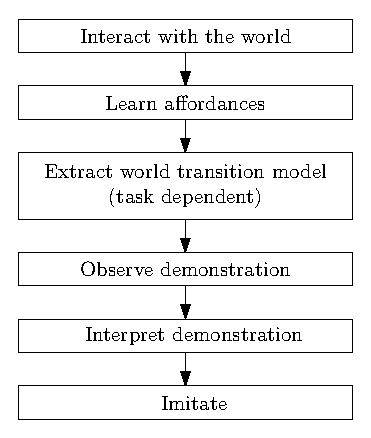
\includegraphics[width=0.3\columnwidth]{images/Diagram.eps}
%Figure 6
\caption{Path to imitation.}
\label{fig:manipulation:path}
\end{figure}

\subsection{Affordance based imitation}
The main objective of acquiring and modeling affordances is to provide
a general model of the world mechanisms in terms of robot actions and
perceptual skills. This model provides a sound base to develop more
complex behaviors. IST has started to explore the use of the
affordance model to develop imitation behaviors. The proposed
framework is shown in Figure~\ref{fig:manipulation:path}. The robot
first learn the affordance network model. Then, it uses this model to
estimate a rough transition model for the proposed task , to extract
information from the demonstrations and translate them into its own
motion repertoire. Using Bayesian inverse reinforcement learning, the
robot interprets the demonstrations and extracts its own policy to
achieve the same goal.

We have conducted some experiments to evaluate the proposed methodology. The robot learned how to sort different objects from a human demonstration (see Figure~\ref{fig:manipulation:experim}(a)).
 
It is important to note that the affordance model only provides a
rough estimate of the transition probabilities between the different
states of the task. In addition to this, the action recognition may
fail. We have done some preliminary studies on the impact of this
errors in the proposed
framework. Figure~\ref{fig:manipulation:experim}(b) shows the impact
of action recognition errors in the learn policy. Although more
studies are needed, the results suggests the proposed framework is
able to cope with the uncertainty and model errors.
%
This work has been published in \cite{montesano:etal:2007}.
\begin{figure}
\begin{tabular}{cc}
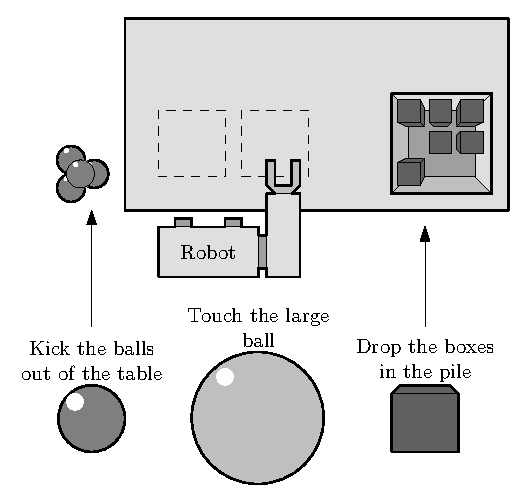
\includegraphics[width=0.45\columnwidth]{images/Recycler.eps} &
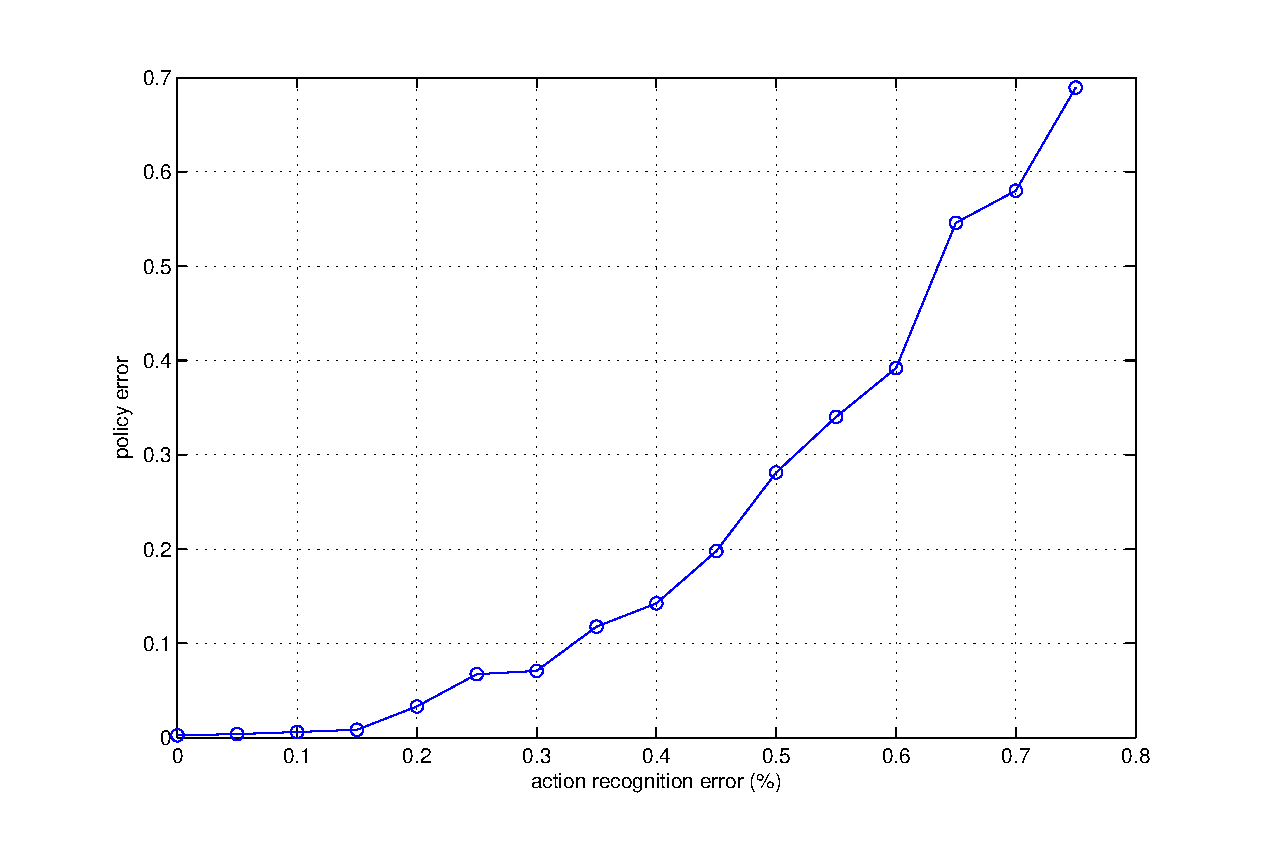
\includegraphics[width=0.45\columnwidth]{images/error.eps} \\
(a) & (b) \\
\end{tabular}
%Figure 7
\caption{Experimental evaluation: (a) setup for imitation learning of
  object sorting, (b) Percentage of wrong actions in the learnt policy
  as the action recognition errors increase.}
\label{fig:manipulation:experim}
\end{figure}

\endinput


\clearpage


\section{Participation in rhythmic events}

As a component of exploratory play, we are interested in giving our
robot the ability to participate in patterned activity in real time
with a human partner.  We include in principle any form of
coordinated motor activity, including vocalization
(singing, proto-dialogue), and gesturing (tapping, dancing).
%
For example, if a human starts humming or tapping something rhythmic, 
we'd like the robot to rapidly join in.

Why is this useful?  Participation in rhythmic activity is a means to
an end, rather than a goal in itself.  The overall goal is to make
machine learning on our robots more autonomous.
%
Knowing the overall structure of an activity gives a ``skeleton'' upon
which the specific objects and actions (potentially initially
unmodeled) within that activity could be analysed.
%
Also, participating in activity is better than just observing it,
since there is an implicit signalling of ``comprehension'' level
available to the human partner, who can reasonably be expected to
adjust their behavior accordingly.


\subsection{Real-time vocal interaction}

The theoretical mechanism was reported in deliverable 1.6.  
UGDIST has made a practical application of that mechanism to
vocal interaction, specifically, to a pitch perception/production
experiment.  We attached prediction to the property of acoustic pitch
as shown in Figure~\ref{fig:sing-module}


\begin{figure}[hbt]
\centerline{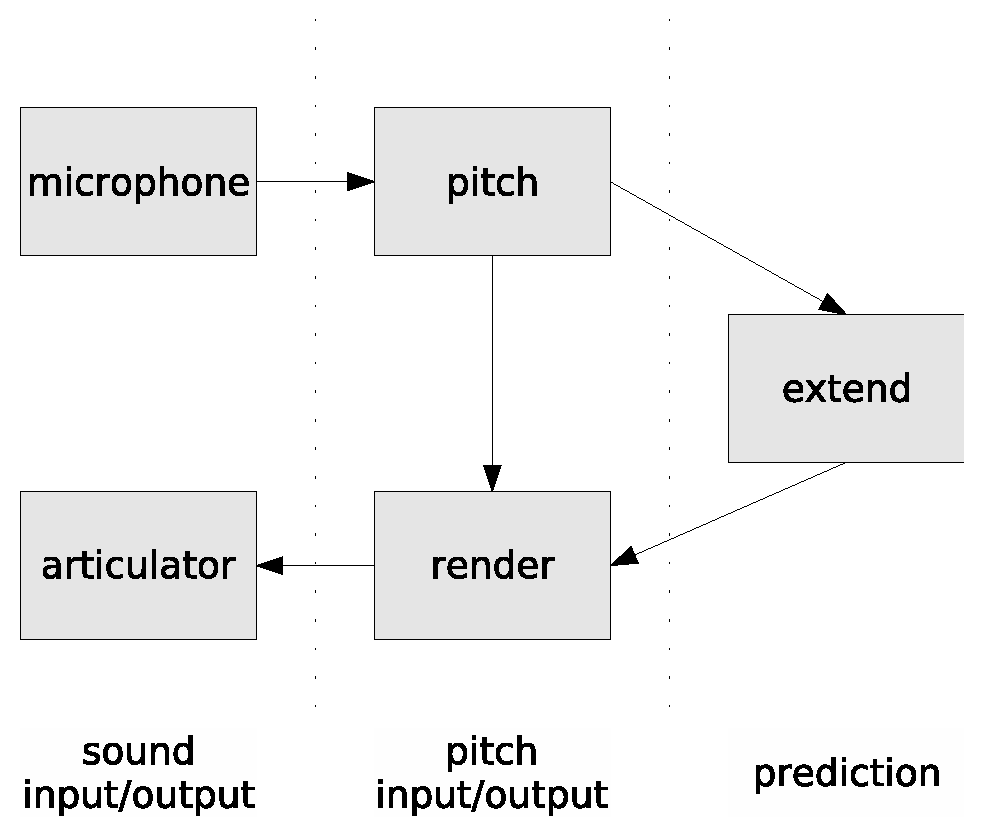
\includegraphics[height=6cm]{images/sing-modules}}
\caption {
%
\label{fig:sing-module}
%
The system for vocal interaction.
The behavior is implemented in the module labelled {\bf render} which
takes the output both of the pitch detector ({\bf pitch}) and a simultaneous 
prediction of what the pitch ``ought'' to be (from {\bf extend})
and decides what sound to make if any.
%
}
\end{figure}

\subsection{Some results}


\begin{figure}[hbt]

\centerline{
a)

\includegraphics[height=2cm]{images/chico-output-separate-high-low}
\ \ 
\ \ 
b)
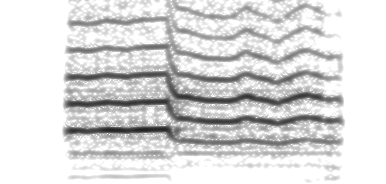
\includegraphics[height=2cm]{images/chico-output-pair-high-low}
\ \ 
\ \ 
c)

\includegraphics[height=2cm]{images/chico-output-ohm}
}

\caption{
%
\label{fig:outcome}
%
Outcome: during a single session the artifact was induced
to generate three distinch patterns of ``speech'': a) two separated
vocalizations with rising pitch; b) a single vocalization with
two tones of falling pitch; and c) a long vocalization of low, steady
pitch.
%
These spectrogram fragments are taken from one continuous session
with the artifact.  Fragments (a) and (b) are generated entirely
by the artifact; fragment (c) is overlaid by sound from
the human partner as well (it was a simultaneous ``meditative chant'').
%
}

\end{figure}





\begin{figure}[hbt]

\centerline{(a) 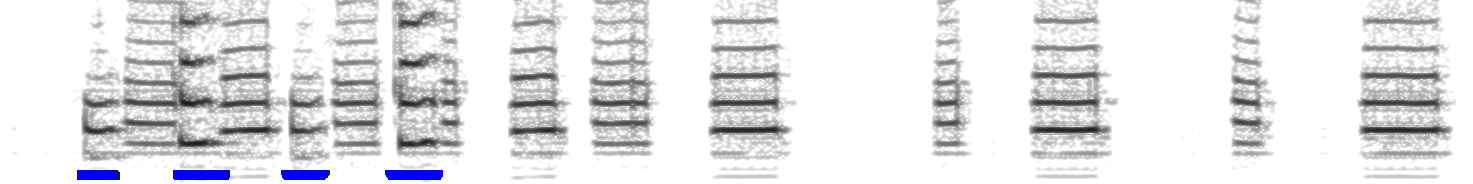
\includegraphics[height=2cm]{images/chico-separate-begin-labelled}}

\ \\

\centerline{(b) 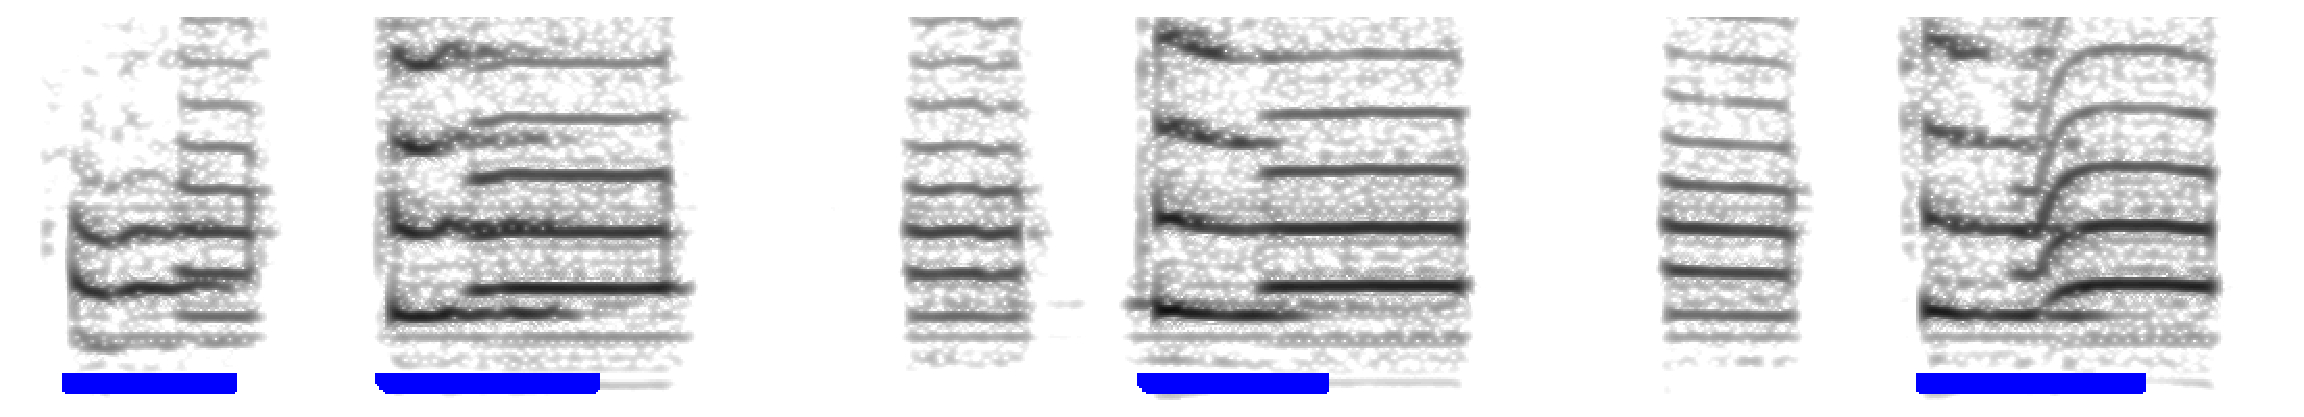
\includegraphics[height=2cm]{images/chico-separate-together-labelled}}

\ \\

\centerline{(c) 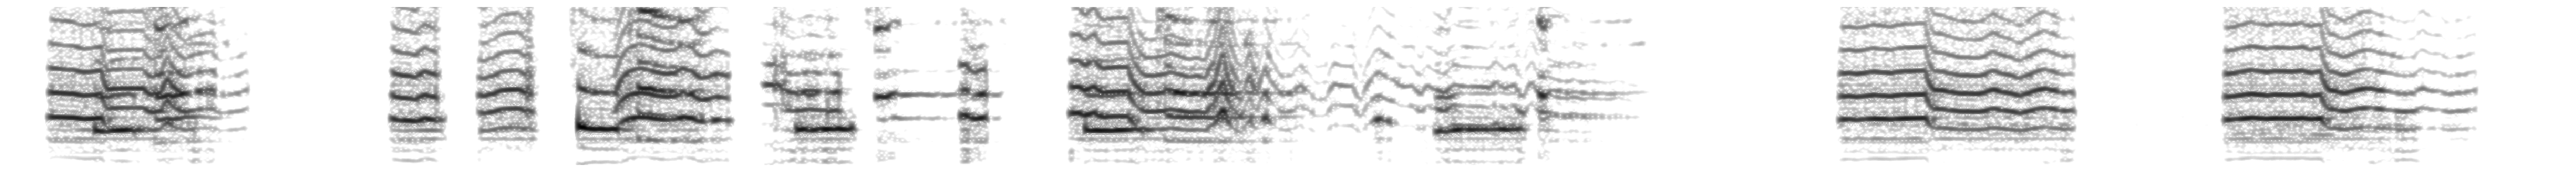
\includegraphics[height=1cm]{images/chico-pair}}

\ \\

\centerline{(d) 
\includegraphics[height=1cm]{images/chico-ohm}}


\caption{
%
Sequence (a) is a spectrogram of the first 14 seconds of human/artifact 
interaction in a 54-second experiment. 
Since we are only concerned with pitch, the 
spectrogram is cropped to emphasis the vertical ``striping'' of 
horizontal lines that reflects the pitch (the greater 
the distance between stripes, the higher the frequency).
The blue bar at the bottom of the spectrogram is added to 
indicate when the human is vocalizing.
%
We see that the human initiates with a short vocalization
and the artifact responds with a short vocalization.  When it
finishes, the human makes a vocalization with a higher pitch.
The artifact responds with a vocalization with a higher pitch.
The human then repeats the first, lower, vocalization.
The artifact responds.  The human repeats the higher vocalization.
The artifact responds with a very abbreviated low tone, then a delay,
then the ``correct'' hight tone.  The human remains silent at this
point, and the robot starts generating a seqence of low and high
tones.
%
Sequence (b) follows on immediately from sequence (a), with 
the human ``joining in'', vocalizating at the same or overlapping time 
as the artifact.  The pattern of vocalization continues low-high,
low-high, like a very simple tune.
%
The tune has been introduced to the artifact without any
explicit or mandatory turn-taking.
%
Sequences (c) and (d) show periods within the same 54-second experiment
where the artifact's behavior is ``shaped'' in the same way
to produce two other tunes.
}

\end{figure}







\subsection{Prosodic unit}


\subsection{Next steps}


\begin{itemize}

\item Apply across multiple signals

\item Different aspects of speech sounds

\item Arm movements, gesturing

\item Exploit knowledge of structure for learning of parts

\end{itemize}




\clearpage


\begin{figure}[bt]
\centerline{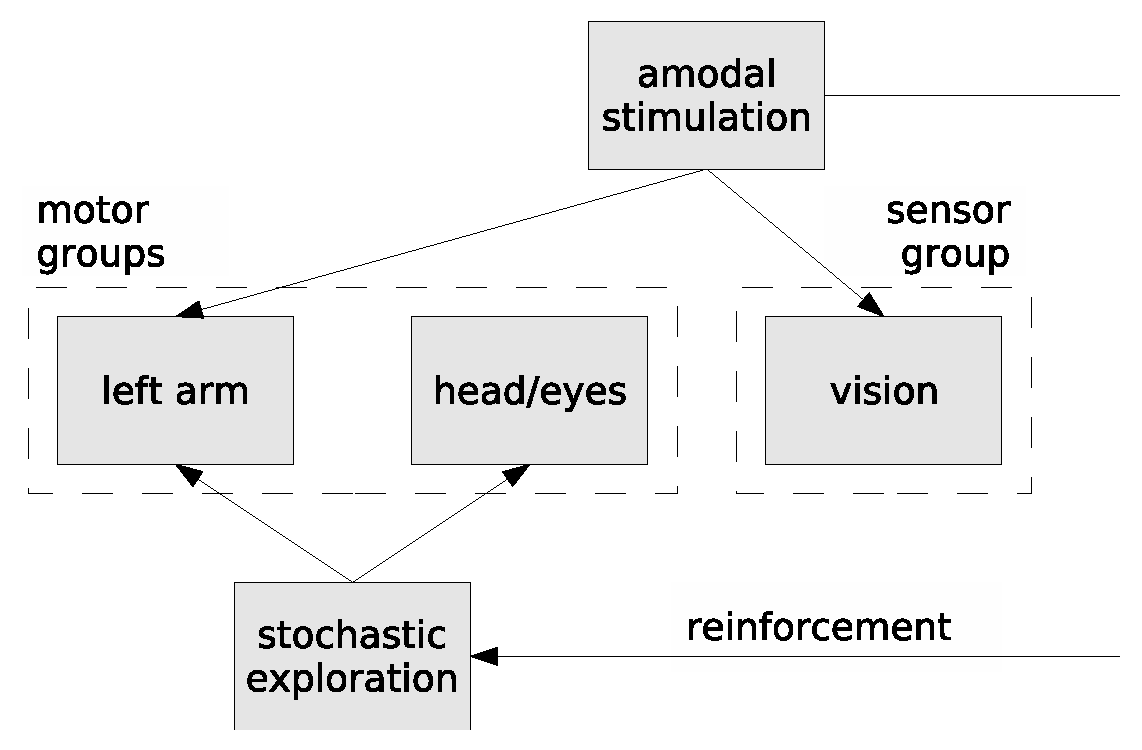
\includegraphics[height=6cm]{images/amodal-modules}}
\caption {
%
\label{fig:amodal-module}
%
The system for stochastic exploration and amodal stimulation.
Exploration exercises a set of motor groups, moving them
to random locations within their nominal ranges.
Amodal stimulation modulates the state of a motor group
in a rhythmic fashion, and looks for signs of that rhythm 
showing up in a sensor group. If the amodal signal does in
fact get transmitted, a reinforcement signal is sent to the
exploration model, biasing further exploration towards the
current configuration of the motor groups.
%
The specific scenario shown here is for visual hand/arm coordination.
The state of the head and arm are explored, while watching for
an amodal connection between the arm and vision.
%
}
\end{figure}

\section{Stochastic exploration and amodal stimulation}

Implemented motor ``babble'' that uses step-wise stochastic search of
the control knobs of a motor system, ``twiddling'' them in a rhythmic
fashion.

Then looks for a ``resonance'' in a specified sensed value
(e.g. visual motion, or clear pitch).  This can be very selective to
the rhythm - helps discount unrelated events.

Gives automatic method for finding configuration of motor system that
produces desired result.


\begin{figure}[p]
\centerline{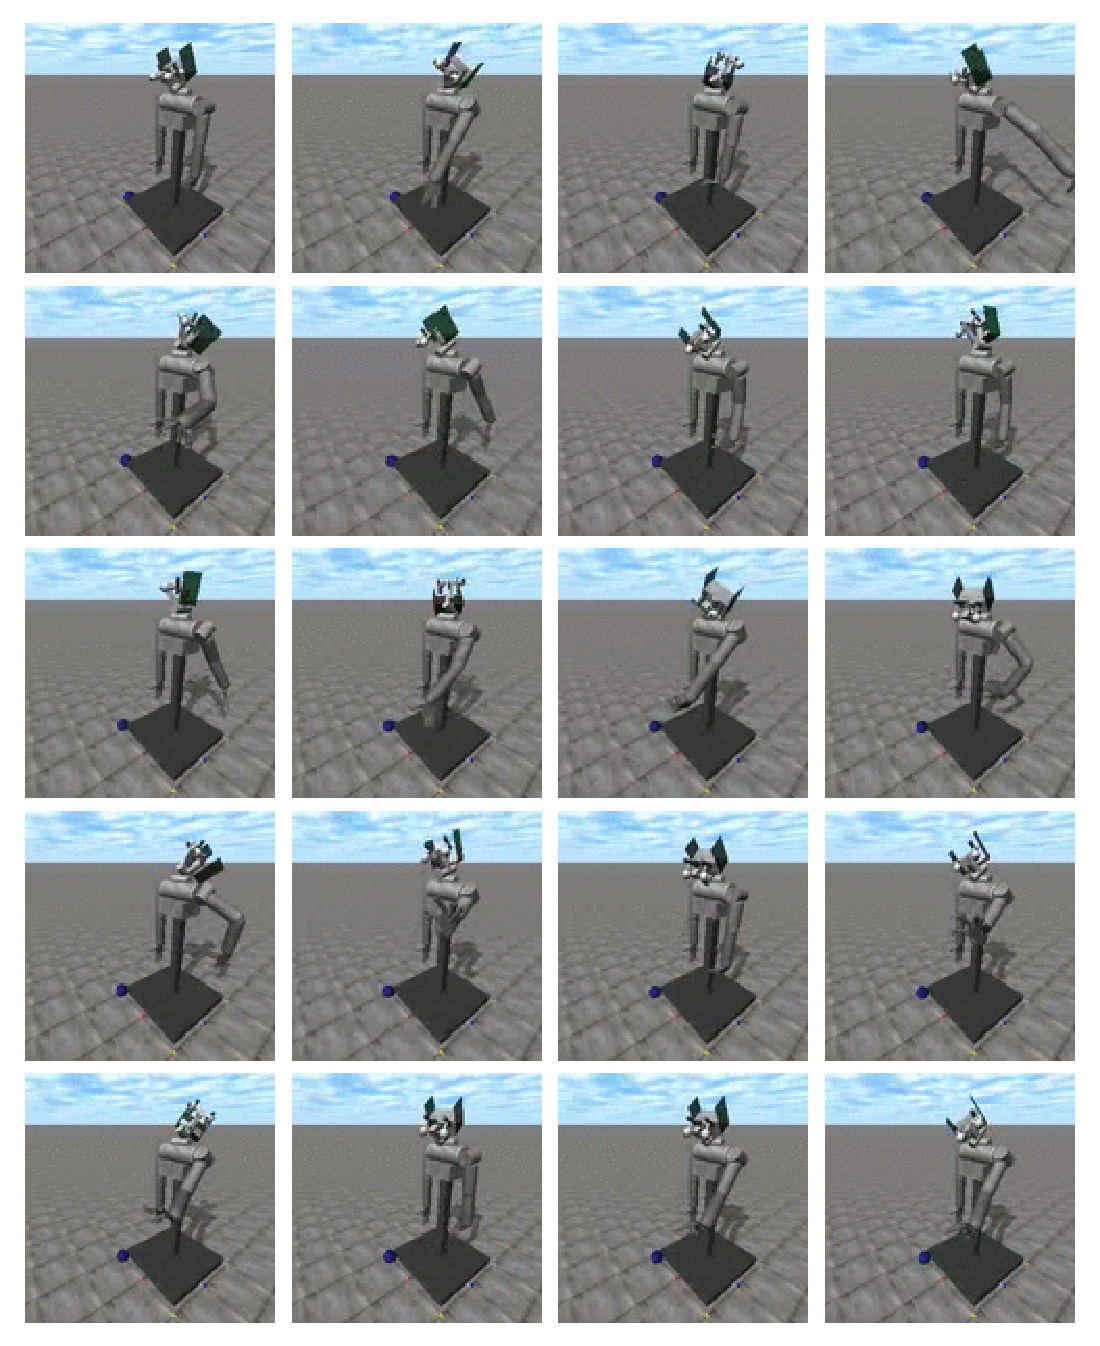
\includegraphics[width=\textwidth]{images/find-arm}}
\caption{
%
A simulated robot, performing motor exploration on its
head/eyes and left arm.  The head, eyes, and arms move around randomly
within their range of movement.
%
A periodic ``shaking'' movement of the arm is made about its
current position, and the effect of this movement is searched 
for visually.
%
When resonance occurs, the configution of head/eyes and left arm
is reinforced so that the robot is more likely to return to that
configuration.
%
This is why 
in early snapshots (top) the robot is unlikely to be looking at 
its arm, and in later snapshots (bottom) the robot is looking at
its arm more often than not.
%
}
\end{figure}

Why?

Want a way of expressing capabilities (such as "bring hand in front of head") in a robust form.

Does NOT assume a tabula rasa - in fact, there is at least as much information involved in exploration (expressing the motor groups to use, their scales, and what sensory cue to monitor) as there would be in just giving numerical pose information.

The difference is robustness to the details of the hand and the head; e.g. could use mirror.

Limitations?

Such stochastic search is very dumb.

Once an initial point of contact has been found, tracking methods would be more efficient for exploring a region of motor space.

Shaking is just one of several amodal cues that could be used (and not a very realistic one)

xref?

Could automate motor space classification examples: gesture recognition, speech recognition

Would have to be a lot simpler than offline, human-mediated work of course.


\subsection{Towards meaning}

The richer the robot's "internal life" is, the more interesting kinds
of "meanings" there can be in its world

- Continuous, broad, shared, structured experience

- Meaning as a process, not a label

Off-line data collection, segmentation, labelling, training of
classifiers, etc work, but restrict the potential semantic universe of
the robot.

For Year 3, online behaviors would be useful.



\clearpage


\bibliographystyle{apalike}
\bibliography{main}


\end{document}
